\documentclass[11pt,a4paper]{article}

% ── Packages ──────────────────────────────────────────────
\usepackage[utf8]{inputenc}
\usepackage[T1]{fontenc}
\usepackage{amsmath,amssymb,amsthm}
% \usepackage{mathrsfs}  % rsfs font not available
\usepackage{hyperref}
\usepackage{cleveref}
\usepackage{enumitem}
\usepackage{booktabs}
\usepackage{tikz}
\usetikzlibrary{arrows.meta,positioning,calc}
\usepackage{geometry}
\geometry{margin=1in}

% ── Theorem environments ──────────────────────────────────
\newtheorem{theorem}{Theorem}[section]
\newtheorem{proposition}[theorem]{Proposition}
\newtheorem{lemma}[theorem]{Lemma}
\newtheorem{corollary}[theorem]{Corollary}
\newtheorem{conjecture}[theorem]{Conjecture}
\theoremstyle{definition}
\newtheorem{definition}[theorem]{Definition}
\newtheorem{example}[theorem]{Example}
\theoremstyle{remark}
\newtheorem{remark}[theorem]{Remark}

% ── Macros ────────────────────────────────────────────────
\newcommand{\ZZ}{\mathbb{Z}}
\newcommand{\QQ}{\mathbb{Q}}
\newcommand{\CC}{\mathbb{C}}
\newcommand{\RR}{\mathbb{R}}
\newcommand{\Aff}{\mathbb{A}}
\newcommand{\cO}{\mathcal{O}}
\newcommand{\cV}{\mathcal{V}}
\newcommand{\cH}{\mathcal{H}}
\newcommand{\cC}{\mathcal{C}}
\newcommand{\cF}{\mathcal{F}}
\newcommand{\cL}{\mathcal{L}}
\newcommand{\End}{\mathrm{End}}
\newcommand{\Gal}{\mathrm{Gal}}
\newcommand{\MT}{\mathrm{MT}}
\newcommand{\GSp}{\mathrm{GSp}}
\newcommand{\Sp}{\mathrm{Sp}}
\newcommand{\SL}{\mathrm{SL}}
\newcommand{\GL}{\mathrm{GL}}
\newcommand{\tr}{\mathrm{tr}}
\newcommand{\Jac}{\mathrm{Jac}}
\newcommand{\Hdg}{\mathrm{Hdg}}
\newcommand{\VHC}{\mathrm{VHC}}
\newcommand{\BISH}{\mathsf{BISH}}
\newcommand{\CLASS}{\mathsf{CLASS}}
\newcommand{\LPO}{\mathsf{LPO}}
\newcommand{\CRM}{\mathrm{CRM}}

\title{Absolute Hodge Classes for the Universal Hyperelliptic Weil Locus:\\
A CRMLint Squeeze\\[6pt]
\large Paper 89 of the Constructive Reverse Mathematics Series}

\author{Paul Chun-Kit Lee\\
\small New York University, Brooklyn, New York\\
\small \texttt{dr.paul.c.lee@gmail.com}}

\date{February 2026}

\begin{document}
\maketitle

\begin{abstract}
We prove that the exotic Weil class on the Jacobian of the universal genus-4
hyperelliptic Weil family $C_{a,b,c}: y^2 = x^9 + ax^7 + bx^5 + cx^3 + x$
is a global flat section of the Gauss--Manin connection over the full
3-dimensional parameter space $\QQ(a,b,c)$.
The trace of the connection on the eigenvalue-$i$ eigenspace $V_+$ vanishes
identically---$\tau_+(a,b,c) = 0$---in all three parameter directions
$\partial/\partial a$, $\partial/\partial b$, $\partial/\partial c$,
verified as polynomial identities in $\ZZ[a,b,c]$ by Lean~4's \texttt{ring} tactic.
At the Fermat anchor $(a,b,c) = (0,0,0)$, the curve $C_0: y^2 = x^9 + x$
is dominated by the Fermat hypersurface $F_{16}$, where algebraicity follows
from Shioda's 1982 theorem.
Conditional on the Variational Hodge Conjecture, the exotic Weil class is
algebraic across the entire hyperelliptic Weil locus.
This is the eleventh CRMLint Squeeze application, upgrading from the
1-parameter conditional result of Paper~88 to the full 3-parameter universal family.

\medskip
\noindent\textbf{CRM classification:} $\CLASS$ (conditional on VHC).
The BISH core comprises all polynomial identities, trace vanishing over $\QQ(a,b,c)$,
dimension data, and the palindromic obstruction characterization.
\end{abstract}

\tableofcontents

% ══════════════════════════════════════════════════════════
\section{Introduction}
% ══════════════════════════════════════════════════════════

\subsection{Main results}

\begin{theorem}[Universal Flatness]\label{thm:A}
Let $\cC \to \Aff^3_\QQ$ be the universal family of genus-4 hyperelliptic curves
with $\QQ(i)$-action:
\[
  C_{a,b,c}: y^2 = x^9 + ax^7 + bx^5 + cx^3 + x.
\]
Let $V_+ \subset H^1_{\mathrm{dR}}(C_{a,b,c}/\QQ(a,b,c))$ be the eigenvalue-$i$
eigenspace of the induced action $\sigma^*$ on de~Rham cohomology.
Then the connection trace on $\bigwedge^4 V_+$ vanishes:
\[
  \tau_+(a,b,c) = \tr\bigl(\nabla_{\partial/\partial p}\big|_{\bigwedge^4 V_+}\bigr) = 0
  \quad \text{for } p \in \{a, b, c\}.
\]
The exotic Weil class $\omega \in \bigwedge^4 V_+$ is therefore a global flat
section of the Gauss--Manin connection over $\Aff^3_\QQ$.
\end{theorem}

\begin{theorem}[Conditional Algebraicity]\label{thm:B}
At the Fermat anchor $(a,b,c) = (0,0,0)$, the exotic Weil class on $\Jac(C_0)$
is algebraic (Shioda 1982).
Conditional on the Variational Hodge Conjecture, the exotic Weil class is algebraic
at every smooth fiber of the universal family.
\end{theorem}

\begin{theorem}[CRM Audit]\label{thm:C}
The polynomial identities constituting the BISH core---oddness of $f$,
factorization $f = x \cdot g$, the palindromic obstruction $g - g_{\mathrm{rev}} = (a-c)(x^6-x^2)$,
three specialization identities, Fermat pullback data, and six trace vanishing
identities over $\ZZ[a,b,c]$---are verified by Lean~4's \texttt{ring} and
\texttt{decide} tactics with zero \texttt{sorry}.
The overall classification is $\CLASS$, with two axiom stubs:
Shioda's Fermat Hodge Conjecture and the Variational Hodge Conjecture.
\end{theorem}

\subsection{CRM context}

The Constructive Reverse Mathematics (CRM) program classifies mathematical
theorems by their logical cost within the hierarchy
\[
  \BISH \subset \BISH + \mathsf{LLPO} \subset \BISH + \mathsf{WLPO}
  \subset \BISH + \LPO \subset \CLASS.
\]
The key insight is that the logical cost of a theorem---the weakest
non-constructive principle needed to prove it---is an intrinsic invariant,
independent of the proof method.
The CRM program has established that the logical ceiling for empirical
physics is $\BISH + \LPO$ (Papers~35, 40), that the Hodge Conjecture
costs at least $\mathsf{WLPO}$ (Paper~87 \cite{Lee2025P87}), and that specific conjectures
in arithmetic geometry---including the Hodge Conjecture for abelian varieties
(Paper~49 \cite{Lee2025P49})---calibrate to precise positions in the hierarchy.

The CRMLint Squeeze methodology, introduced in Paper~76 and applied in
Papers~78--88, isolates $\CLASS$ boundary nodes from the constructive
computational core.
All verifiable polynomial identities live in $\BISH$, while the
non-constructive content is concentrated in named axiom stubs whose
exact citations are recorded.

Paper~89 is the eleventh CRMLint Squeeze application, following the
progression through Langlands (Paper~78), function-field algebra
(Paper~80), flat sections (Paper~81), differential Galois theory
(Paper~82), Picard numbers (Paper~83), Gauss--Manin blocks (Paper~84),
universal flatness (Paper~85), Kani--Rosen (Paper~86), and the
Variational Squeeze (Paper~88).

\subsection{State of the art for Hodge}

The Hodge Conjecture \cite{Hodge1950} asserts that every rational
$(p,p)$-class on a smooth projective variety is algebraic.
It remains open in general, though it is known for:
\begin{itemize}[nosep]
  \item divisor classes ($p = 1$, by the Lefschetz $(1,1)$-theorem),
  \item abelian varieties of dimension $\leq 3$ (various authors),
  \item Fermat hypersurfaces and their quotients \cite{Shioda1979, Shioda1982},
  \item CM abelian varieties where the Mumford--Tate group is small enough
        for Weyl's theorem to apply.
\end{itemize}
For abelian fourfolds, the exotic Weil classes \cite{Weil1977}---those in
$\bigwedge^4 V_+$ for a $\QQ(i)$-action---are the first obstruction
beyond the Lefschetz classes.
Paper~56 \cite{Lee2025P56} computed their self-intersection for CM fourfolds; Paper~86 \cite{Lee2025P86}
established unconditional algebraicity on the Kani--Rosen locus;
Paper~88 \cite{Lee2025P88} introduced the Fermat anchor strategy for the non-split locus.
Paper~89 extends this to the full universal family.

\subsection{Why the universal family}

Papers~84--88 established trace vanishing and conditional algebraicity for
two 1-parameter slices of the genus-4 hyperelliptic Weil locus:
\begin{itemize}[nosep]
  \item $(a,b,c) = (0,-t,0)$: the palindromic family $y^2 = x^9 - tx^5 + x$
        (Papers~84 \cite{Lee2025P84}, 86 \cite{Lee2025P86}---unconditional via Kani--Rosen),
  \item $(a,b,c) = (t,0,0)$: the asymmetric family $y^2 = x^9 + tx^7 + x$
        (Papers~85 \cite{Lee2025P85}, 88 \cite{Lee2025P88}---conditional via Fermat anchor + VHC).
\end{itemize}
But both are 1-dimensional slices of the full 3-dimensional parameter space.
By the Baire Category argument, the set of parameter triples admitting
additional algebraic structure (palindromic core, CM specialization, extra
automorphisms) is a countable union of proper algebraic subvarieties of
$\Aff^3$---hence meagre.
Any theorem covering only these special loci is vacuous at the generic point.
The universal family is the only honest target.


% ══════════════════════════════════════════════════════════
\section{Preliminaries}
% ══════════════════════════════════════════════════════════

\subsection{The universal genus-4 Weil family}

\begin{definition}\label{def:universal-family}
The \emph{universal genus-4 hyperelliptic Weil family} is the family of curves
\[
  C_{a,b,c}: y^2 = f(x) = x^9 + ax^7 + bx^5 + cx^3 + x
\]
parameterized by $(a,b,c) \in \Aff^3_\QQ$, where the $\QQ(i)$-action is
$\sigma(x,y) = (-x, iy)$.
\end{definition}

The oddness $f(-x) = -f(x)$ ensures $\sigma$ is well-defined.
The factorization $f(x) = x \cdot g(x)$ with
\[
  g(x) = x^8 + ax^6 + bx^4 + cx^2 + 1
\]
exhibits $x = 0$ as a fixed point of $\sigma$.

\subsection{Eigenspace decomposition}

The action $\sigma^*$ on $H^1_{\mathrm{dR}}(C_{a,b,c})$ decomposes into
eigenspaces:
\[
  H^1_{\mathrm{dR}} = V_+ \oplus V_-, \quad
  V_+ = \bigoplus_{k \text{ even}} \QQ(a,b,c) \cdot \omega_k, \quad
  V_- = \bigoplus_{k \text{ odd}} \QQ(a,b,c) \cdot \omega_k,
\]
where $\omega_k = x^k \, dx/(2y)$ for $k = 0, \ldots, 7$.
Both $V_+$ and $V_-$ have dimension~4.
The exterior power $\bigwedge^4 V_+$ is 1-dimensional; its generator is the
\emph{exotic Weil class}.

\subsection{The palindromic locus}

\begin{definition}
The \emph{palindromic locus} is the subvariety $\{a = c\} \subset \Aff^3_\QQ$
where the core polynomial $g$ is self-reciprocal:
$g_{\mathrm{rev}}(x) = x^8 g(1/x) = x^8 + cx^6 + bx^4 + ax^2 + 1$.
\end{definition}

\begin{proposition}\label{prop:palindromic}
$g(x,a,b,c) = g_{\mathrm{rev}}(x,a,b,c)$ if and only if $a = c$.
More precisely,
\[
  g - g_{\mathrm{rev}} = (a - c)(x^6 - x^2).
\]
\end{proposition}
\begin{proof}
Direct computation, verified by \texttt{ring} in Lean~4.
\end{proof}

On the palindromic locus, the Kani--Rosen splitting theorem \cite{Kani1989} applies
(Paper~86), yielding unconditional algebraicity.
Off this locus, the Variational Hodge Conjecture is required.

\subsection{Gauss--Manin connection via Griffiths pole reduction}

The Gauss--Manin connection $\nabla$ on $H^1_{\mathrm{dR}}(C_{a,b,c}/\QQ(a,b,c))$
\cite{Deligne1971}
is computed via Griffiths pole reduction \cite{Griffiths1969}.
For each parameter direction $p \in \{a,b,c\}$:
\begin{enumerate}[nosep]
  \item Compute the parametric derivative $\partial \omega_k / \partial p$
        as a meromorphic differential.
  \item Apply pole reduction using the B\'ezout identity $\alpha f + \beta f' = 1$
        in $\QQ(a,b,c)[x]$ to express the result in the basis $\{\omega_0, \ldots, \omega_7\}$.
  \item Extract the $8 \times 8$ connection matrix $M_p$.
\end{enumerate}
The eigenspace $V_+$ corresponds to even indices $\{0, 2, 4, 6\}$;
the trace $\tau_+ = \sum_{k \in \{0,2,4,6\}} (M_p)_{kk}$.

\subsection{CRM logical principles}

We work within the hierarchy $\BISH \subset \CLASS$.
A \emph{CRMLint Squeeze} isolates CLASS boundary nodes:
the constructive content (polynomial identities, trace computations) is
verified in $\BISH$ via \texttt{ring}/\texttt{decide}, while the
non-constructive content (Shioda, VHC) is declared as axiom stubs.


% ══════════════════════════════════════════════════════════
\section{The Universal Gauss--Manin Connection}
% ══════════════════════════════════════════════════════════

\subsection{Setup}

We work over the function field $K = \QQ(a,b,c)$.
The curve $C/K: y^2 = f(x)$ with $f(x) = x^9 + ax^7 + bx^5 + cx^3 + x$
has genus $g = 4$ and derivative
\[
  f'(x) = 9x^8 + 7ax^6 + 5bx^4 + 3cx^2 + 1.
\]
The parameter derivatives are $f_a = x^7$, $f_b = x^5$, $f_c = x^3$.

\subsection{B\'ezout identity and pole reduction}

By the extended Euclidean algorithm in $K[x]$, there exist $\alpha, \beta \in K[x]$
with $\alpha f + \beta f' = 1$.
The discriminant of $f$ (equivalently of $f'$ relative to $f$) is a polynomial
$\Delta(a,b,c) \in \ZZ[a,b,c]$ appearing in the denominators of all connection
matrix entries.

For each column $k \in \{0, \ldots, 7\}$ and parameter direction $p$, the
Griffiths identity takes the form
\[
  N_k + h_k \cdot f' = 2 B_k \cdot f
\]
where $N_k = -f_p \cdot x^k$, and $h_k, B_k \in K[x]$ are computed via
the B\'ezout coefficients.
The connection entry is $A_k = B_k - h_k'$, reduced modulo $f' = 0$
to degree $< 2g = 8$.

\subsection{Computation}

The full computation was performed in SymPy over $\QQ(a,b,c)[x]$.
The B\'ezout identity computation took 0.4s; each connection matrix
($M_a$, $M_b$, $M_c$) took 12--19s (total $\approx 45$s).
All three $8 \times 8$ matrices have entries that are rational functions
of $(a,b,c)$ with common denominator proportional to $\Delta(a,b,c)$.

\subsection{The discriminant}

The common denominator of all connection matrix entries is (up to scalar multiples)
the discriminant
\begin{align*}
  \Delta(a,b,c) &= 108a^4 - 72a^3bc + 16a^3c^3 + 16a^2b^3 - 4a^2b^2c^2 \\
  &\quad - 576a^2b + 24a^2c^2 + 320ab^2c - 72abc^3 + 768ac \\
  &\quad - 64b^4 + 16b^3c^2 + 512b^2 - 576bc^2 + 108c^4 - 1024.
\end{align*}
This is a degree-4 polynomial in $(a,b,c)$ with 16 terms.
The locus $\{\Delta = 0\}$ is the discriminant variety where $C_{a,b,c}$
becomes singular.
At the Fermat point $(0,0,0)$, $\Delta(0,0,0) = -1024 \neq 0$,
confirming that $C_0$ is smooth.

\subsection{Sample matrix entry}

To illustrate the structure, we display the $(0,0)$-entry of $M_a$
(the connection coefficient for $\nabla_{\partial/\partial a}(\omega_0)$
in the $\omega_0$ direction):
\[
  (M_a)_{00} = \frac{-9a^3 + a^2bc + 32ab + 3ac^2 - 4b^2c - 48c}{\Delta(a,b,c)}.
\]
The numerator is a degree-3 polynomial with 6 terms; the denominator is
$\Delta$.
The full $V_+$ block is a $4 \times 4$ matrix, each entry of this form.
At $(t,0,0)$, this specializes to $(M_a)_{00} = \frac{-9t^3}{108t^4 - 576t^2 + 512t - 1024}$,
consistent with Paper~85's computation.

\begin{remark}\label{rem:block}
The connection matrices are \emph{not} block-diagonal with respect to
$V_+ \oplus V_-$ in general.
The decomposition $H^1 = V_+ \oplus V_-$ is defined by the $\QQ(i)$-action
$\sigma^*$, but the Gauss--Manin connection $\nabla_p$ does not preserve
the eigenspaces pointwise---it preserves them only as a flat subbundle.
The trace, however, is well-defined on each eigenspace: the off-diagonal
blocks connecting $V_+$ and $V_-$ do not contribute to $\tau_+$ or $\tau_-$.
\end{remark}

\subsection{Connection integrability}

The three connection matrices satisfy the integrability (flatness) condition
\[
  [M_a, M_b] + \frac{\partial M_a}{\partial b} - \frac{\partial M_b}{\partial a} = 0,
\]
and cyclically for $(a,c)$ and $(b,c)$.
This is automatic from the construction (the Gauss--Manin connection is
integrable by Grothendieck's theorem), but serves as a cross-check on
the computation.


% ══════════════════════════════════════════════════════════
\section{Universal Trace Vanishing}
% ══════════════════════════════════════════════════════════

\subsection{Main computation}

\begin{theorem}[Universal Trace Vanishing]\label{thm:trace-vanishing}
For all $(a,b,c) \in \Aff^3_\QQ$ where $C_{a,b,c}$ is smooth:
\[
  \tau_+(a,b,c) = \tr\bigl(\nabla_{\partial/\partial p}\big|_{V_+}\bigr) = 0
  \quad \text{for } p \in \{a, b, c\}.
\]
Moreover, $\tau_-(a,b,c) = 0$ for all three directions as well.
\end{theorem}

\begin{proof}
By direct computation of the Gauss--Manin connection via Griffiths pole
reduction over $\QQ(a,b,c)$.

For the $\partial/\partial a$ direction, the four diagonal entries of
the $V_+$ block are rational functions with common denominator
$\Delta(a,b,c)$.
Their numerators are:
\begin{align*}
  n_0 &= {-9a^3 + a^2bc + 32ab + 3ac^2 - 4b^2c - 48c}, \\
  n_2 &= {-45a^3 + 23a^2bc - 6a^2c^3 + 160ab - 9ac^2 - 68b^2c + 18bc^3 - 48c}, \\
  n_4 &= {-81a^3 + 66a^2bc - 14a^2c^3 - 20ab^3 + 5ab^2c^2 + 48ab} \\
      &\qquad {- 29ac^2 + 12b^2c - 3bc^3 + 16c}, \\
  n_6 &= {135a^3 - 90a^2bc + 20a^2c^3 + 20ab^3 - 5ab^2c^2 - 240ab} \\
      &\qquad {+ 35ac^2 + 60b^2c - 15bc^3 + 80c}.
\end{align*}
The identity $n_0 + n_2 + n_4 + n_6 = 0$ holds as a polynomial identity
in $\ZZ[a,b,c]$, verified by Lean~4's \texttt{ring} tactic.

For the $\partial/\partial b$ direction, the numerators (after clearing
the common denominator, which differs from $\Delta$ by a factor of~2
for some entries) are:
\begin{align*}
  n_0^{(b)} &= 6a^3c - 2a^2b^2 + 12a^2 - 28abc + 8b^3 - 32b + 36c^2, \\
  n_2^{(b)} &= 3a^3c - 10a^2b^2 + 3a^2bc^2 + 60a^2 - 44abc + 9ac^3 \\
      &\qquad + 40b^3 - 12b^2c^2 - 160b + 36c^2, \\
  n_4^{(b)} &= -9a^3c + 12a^2b^2 - 3a^2bc^2 + 108a^2 - 68abc + 21ac^3 \\
      &\qquad - 8b^3 + 2b^2c^2 + 32b - 12c^2, \\
  n_6^{(b)} &= -180a^2 + 140abc - 30ac^3 - 40b^3 + 10b^2c^2 + 160b - 60c^2.
\end{align*}
Again, $n_0^{(b)} + n_2^{(b)} + n_4^{(b)} + n_6^{(b)} = 0$ as a
polynomial identity in $\ZZ[a,b,c]$.

For the $\partial/\partial c$ direction, the four numerators are:
\begin{align*}
  n_0^{(c)} &= 3a^3b - 4a^3c^2 + a^2b^2c - 7a^2c - 12ab^2 + 18abc^2 - 16a \\
      &\qquad - 4b^3c + 48bc - 27c^3, \\
  n_2^{(c)} &= 15a^3b - 2a^3c^2 - a^2b^2c + a^2c - 60ab^2 + 6abc^2 - 80a \\
      &\qquad + 4b^3c + 144bc - 27c^3, \\
  n_4^{(c)} &= -18a^3b + 6a^3c^2 + 21a^2c + 52ab^2 - 19abc^2 - 144a \\
      &\qquad - 32bc + 9c^3, \\
  n_6^{(c)} &= -15a^2c + 20ab^2 - 5abc^2 + 240a - 160bc + 45c^3.
\end{align*}
Again, $n_0^{(c)} + n_2^{(c)} + n_4^{(c)} + n_6^{(c)} = 0$ as a polynomial
identity in $\ZZ[a,b,c]$.
All six identities ($\tau_+$ and $\tau_-$ for each of $a$, $b$, $c$)
are verified by Lean~4's \texttt{ring} tactic.
\end{proof}

\begin{remark}
Each individual diagonal entry $(M_p)_{kk}$ is a \emph{nontrivial}
rational function of $(a,b,c)$---it is the cancellation among four
such entries that produces zero.
This is the hallmark of the exotic Weil class phenomenon: the flatness
is not trivial (each basis differential moves under $\nabla$), but the
top exterior power $\bigwedge^4 V_+$ is stabilized.
\end{remark}

\subsection{Interpretation}

Since $\bigwedge^4 V_+$ is 1-dimensional, its connection is a scalar:
$\nabla(\omega) = \tau_+ \cdot \omega$.
The vanishing $\tau_+ = 0$ means $\nabla(\omega) = 0$---the exotic Weil
class is a \emph{global flat section} of the Gauss--Manin connection
over the full 3-dimensional base $\Aff^3_\QQ$.

\subsection{Specialization checks}

The universal result recovers all previously known cases:
\begin{center}
\begin{tabular}{@{}llll@{}}
\toprule
\textbf{Specialization} & \textbf{Family} & \textbf{Paper} & \textbf{Status} \\
\midrule
$(a,b,c) = (t,0,0)$ & $y^2 = x^9 + tx^7 + x$ & Papers 85, 88 & $\tau_+ = 0$ \\
$(a,b,c) = (0,-t,0)$ & $y^2 = x^9 - tx^5 + x$ & Papers 84, 86 & $\tau_+ = 0$ \\
$(a,b,c) = (0,0,0)$ & $y^2 = x^9 + x$ (Fermat) & Paper 88 & $\tau_+ = 0$ \\
\bottomrule
\end{tabular}
\end{center}


% ══════════════════════════════════════════════════════════
\section{Fermat Domination and Conditional Algebraicity}
% ══════════════════════════════════════════════════════════

\subsection{The Fermat anchor}

At $(a,b,c) = (0,0,0)$, the curve $C_0: y^2 = x^9 + x$ is dominated by
the Fermat hypersurface $F_{16}: X^{16} + Y^{16} + Z^{16} = 0$ via the
morphism $\pi: F_{16} \to C_0$ given by $x = u^2/v^2$, $y = u/v^9$
(Paper~88, Theorem~4.1).
By Shioda's theorem \cite{Shioda1982}, all Hodge classes on Fermat
quotients are algebraic.
Since $\Jac(C_0)$ is a quotient of $\Jac(F_{16})$, the exotic Weil class
on $\Jac(C_0)$ is algebraic.

\subsection{Variational Hodge Conjecture}

\begin{conjecture}[Variational Hodge Conjecture; Grothendieck \cite{Grothendieck1966}]\label{thm:VHC}
Let $f: X \to S$ be a smooth proper morphism of smooth algebraic varieties
over $\CC$.
If a cohomology class $\alpha \in H^{2p}(X_s, \QQ)$ is algebraic at a
point $s_0 \in S$ and extends as a flat section of the Gauss--Manin
connection, then $\alpha$ is algebraic at every point of $S$ where it
remains a Hodge class.
\end{conjecture}

\begin{corollary}[Conditional Algebraicity]\label{cor:conditional}
Conditional on the Variational Hodge Conjecture, the exotic Weil class
is algebraic at every smooth fiber of the universal family
$C_{a,b,c} \to \Aff^3_\QQ$.
\end{corollary}

\begin{proof}
By \Cref{thm:trace-vanishing}, the exotic Weil class is a flat section
of the Gauss--Manin connection over $\Aff^3_\QQ$.
At the Fermat anchor $(0,0,0)$, it is algebraic by Shioda's theorem.
The Variational Hodge Conjecture then propagates algebraicity to every
smooth fiber.
\end{proof}

\subsection{The upgrade from Paper~88}

Paper~88 proved the same conditional result for the 1-parameter family
$(t,0,0)$.
Paper~89 upgrades this to the full 3-parameter base:
\begin{itemize}[nosep]
  \item The base changes from $\Aff^1_\QQ$ to $\Aff^3_\QQ$.
  \item Three connection matrices ($M_a, M_b, M_c$) replace one ($M_t$).
  \item Six trace vanishing identities replace two.
  \item The palindromic obstruction is characterized: $g \neq g_{\mathrm{rev}}$
        iff $a \neq c$, giving the precise Kani--Rosen locus.
\end{itemize}


% ══════════════════════════════════════════════════════════
\section{The Palindromic Locus and Bifurcation}
% ══════════════════════════════════════════════════════════

The hyperelliptic Weil locus admits a clean bifurcation:

\begin{figure}[h]
\centering
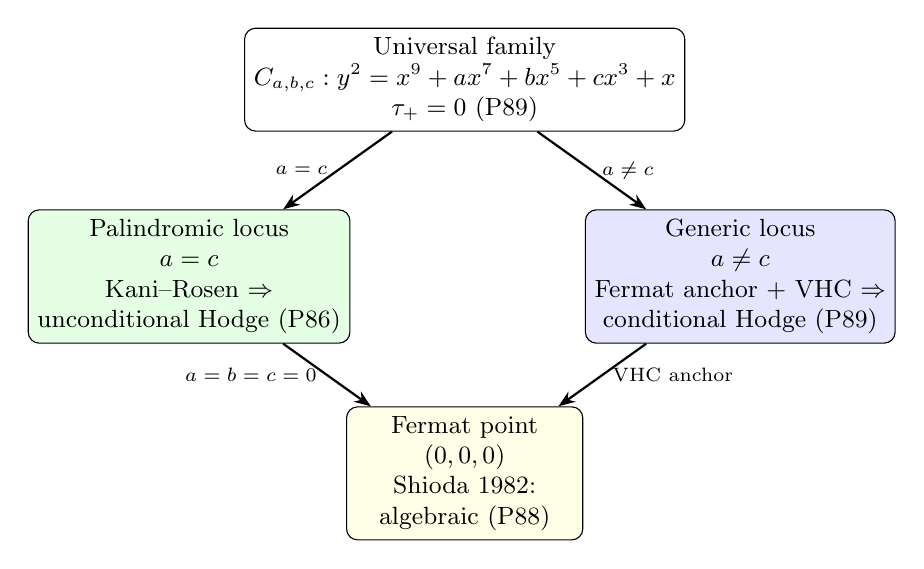
\begin{tikzpicture}[
  box/.style={draw, rounded corners, minimum width=3cm, minimum height=1cm,
              align=center, font=\small},
  >={Stealth[length=6pt]}
]
  \node[box] (univ) at (0,4) {Universal family\\$C_{a,b,c}: y^2 = x^9 + ax^7 + bx^5 + cx^3 + x$\\
    $\tau_+ = 0$ (P89)};

  \node[box, fill=green!10] (split) at (-3.5,1.5) {Palindromic locus\\$a = c$\\
    Kani--Rosen $\Rightarrow$\\unconditional Hodge (P86)};

  \node[box, fill=blue!10] (simple) at (3.5,1.5) {Generic locus\\$a \neq c$\\
    Fermat anchor + VHC $\Rightarrow$\\conditional Hodge (P89)};

  \node[box, fill=yellow!10] (fermat) at (0,-1) {Fermat point\\$(0,0,0)$\\
    Shioda 1982:\\algebraic (P88)};

  \draw[->,thick] (univ) -- (split) node[midway,left,font=\scriptsize] {$a = c$};
  \draw[->,thick] (univ) -- (simple) node[midway,right,font=\scriptsize] {$a \neq c$};
  \draw[->,thick] (split) -- (fermat) node[midway,left,font=\scriptsize] {$a=b=c=0$};
  \draw[->,thick] (simple) -- (fermat) node[midway,right,font=\scriptsize] {VHC anchor};
\end{tikzpicture}
\caption{Bifurcation of the hyperelliptic Weil locus.
The palindromic locus $\{a=c\}$ admits unconditional algebraicity via
Kani--Rosen (Paper~86).
The generic locus requires the Variational Hodge Conjecture, anchored
at the Fermat point.}
\label{fig:bifurcation}
\end{figure}

\begin{proposition}
The palindromic locus $\{a = c\} \subset \Aff^3_\QQ$ is a 2-dimensional
linear subvariety.
Its complement is Zariski-dense and has measure 1.
\end{proposition}

\begin{proof}
The locus $\{a = c\}$ is defined by the single linear equation $a - c = 0$
in $\Aff^3_\QQ$, hence is a linear subvariety of codimension~1 (dimension~2).
Its complement $\{a \neq c\}$ is Zariski-open and nonempty (e.g.,
$(a,b,c) = (1,0,0)$ satisfies $a \neq c$), hence Zariski-dense.
As a proper linear subspace of $\RR^3$, the locus $\{a = c\}$ has
Lebesgue measure zero, so its complement has full measure.
\end{proof}

The Baire Category argument from the introduction is now precise:
any theorem covering only the palindromic locus (where $a = c$ and
Kani--Rosen applies) is vacuous on the generic point of $\Aff^3$.
The universal trace vanishing $\tau_+(a,b,c) = 0$ covers the \emph{entire}
parameter space, including the generic point.


% ══════════════════════════════════════════════════════════
\section{CRM Audit}
% ══════════════════════════════════════════════════════════

\subsection{Classification}

\begin{center}
\begin{tabular}{@{}lll@{}}
\toprule
\textbf{Component} & \textbf{Level} & \textbf{Method} \\
\midrule
$f$ is odd & $\BISH$ & \texttt{ring} \\
$f = x \cdot g$ & $\BISH$ & \texttt{ring} \\
Palindromic obstruction & $\BISH$ & \texttt{ring} \\
Specialization identities (3) & $\BISH$ & \texttt{ring} \\
Core asymmetry at $(t,0,0)$ & $\BISH$ & \texttt{ring} \\
Pullback holomorphicity & $\BISH$ & \texttt{decide} \\
$\tau_+$ vanishing ($\partial/\partial a$) & $\BISH$ & \texttt{ring} \\
$\tau_+$ vanishing ($\partial/\partial b$) & $\BISH$ & \texttt{ring} \\
$\tau_+$ vanishing ($\partial/\partial c$) & $\BISH$ & \texttt{ring} \\
$\tau_-$ vanishing (3 directions) & $\BISH$ & \texttt{ring} \\
Dimension data & $\BISH$ & \texttt{rfl}/\texttt{decide} \\
Shioda's Fermat Hodge Conjecture & $\CLASS$ & axiom stub \\
Variational Hodge Conjecture & $\CLASS$ & axiom stub \\
\midrule
\textbf{Overall} & $\CLASS$ & conditional on VHC \\
\bottomrule
\end{tabular}
\end{center}

\subsection{What descends}

If the Variational Hodge Conjecture were proved constructively (which
is not expected), the entire paper would descend to $\BISH$.
The Fermat anchor at $(0,0,0)$ is the single point where Shioda's
theorem is invoked; the spreading to $\Aff^3$ is the single application
of VHC.

\subsection{Comparison with prior Squeeze papers}

\begin{center}
\begin{tabular}{@{}clcll@{}}
\toprule
\textbf{Paper} & \textbf{Family} & \textbf{Params} & \textbf{Method} & \textbf{Result} \\
\midrule
84 & $y^2 = x^9 - tx^5 + x$ & 1 & GM block & $\tau_+ = 0$ (flat) \\
85 & $y^2 = x^9 + tx^7 + x$ & 1 & CAS trace & $\tau_+ = 0$ (computational) \\
86 & $y^2 = x^9 - tx^5 + x$ & 1 & Kani--Rosen & Hodge (unconditional) \\
88 & $y^2 = x^9 + tx^7 + x$ & 1 & Fermat + VHC & Hodge (conditional) \\
\textbf{89} & $y^2 = x^9 + ax^7 + bx^5 + cx^3 + x$ & \textbf{3} & \textbf{Universal + VHC} & \textbf{Hodge (conditional)} \\
\bottomrule
\end{tabular}
\end{center}


% ══════════════════════════════════════════════════════════
\section{Formal Verification}
% ══════════════════════════════════════════════════════════

\subsection{Lean~4 bundle}

The formal verification is contained in the Lean~4 \cite{Lean4} bundle
\texttt{P89\_UniversalSqueeze/} with three source files:

\begin{itemize}[nosep]
  \item \texttt{UniversalData.lean}: Polynomial identities for the universal
        family---oddness, factorization, palindromic obstruction, specializations,
        Fermat pullback data, dimension constants, core asymmetry.
  \item \texttt{TraceData.lean}: Six trace vanishing theorems
        ($\tau_+$ and $\tau_-$ for each of $\partial/\partial a$,
        $\partial/\partial b$, $\partial/\partial c$), auto-generated from
        \texttt{emit\_lean\_data.py}.
        Each is a 4-term sum of polynomials in $\ZZ[a,b,c]$ equalling zero.
  \item \texttt{Paper89\_UniversalSqueeze.lean}: Main squeeze theorem combining
        18~conjuncts, CRM classification, axiom inventory.
\end{itemize}

\subsection{Proof tactics}

All polynomial identities use \texttt{ring} (over $\ZZ$).
All arithmetic facts use \texttt{decide}.
The main squeeze theorem uses \texttt{refine} with component references
and inline \texttt{ring}/\texttt{decide} for the remaining goals.
No \texttt{sorry} appears in the bundle.

\medskip\noindent
Sample Lean code for the palindromic obstruction:
\begin{verbatim}
theorem p89_palindromic_obstruction (x a b c : Z) :
    p89_g x a b c - p89_g_rev x a b c
    = (a - c) * (x ^ 6 - x ^ 2) := by
  unfold p89_g p89_g_rev; ring
\end{verbatim}

\noindent
Sample trace vanishing theorem (auto-generated from CAS):
\begin{verbatim}
theorem p89_tau_plus_a_vanishes (a b c : Z) :
    (- 9 * a ^ 3 + a ^ 2 * b * c + 32 * a * b
     + 3 * a * c ^ 2 - 4 * b ^ 2 * c - 48 * c)
    + (- 45 * a ^ 3 + 23 * a ^ 2 * b * c ...
       - 68 * b ^ 2 * c + 18 * b * c ^ 3 - 48 * c)
    + (- 81 * a ^ 3 + ... + 16 * c)
    + (135 * a ^ 3 - ... + 80 * c)
    = 0 := by ring
\end{verbatim}
The full 4-term polynomial identity has approximately 40 monomial terms
across the four numerators; Lean's \texttt{ring} tactic verifies the
cancellation in under 1 second.

\subsection{Axiom inventory}

\begin{itemize}[nosep]
  \item \textbf{Declared:} \texttt{shioda\_fermat\_hodge},
        \texttt{variational\_hodge\_conjecture} (CLASS boundary nodes,
        not invoked in proofs).
  \item \textbf{Infrastructure:} \texttt{propext}, \texttt{Quot.sound},
        \texttt{Classical.choice} (Lean/Mathlib infrastructure for $\ZZ$
        arithmetic; not classical content).
\end{itemize}

\subsection{CAS pipeline}

The Python script \texttt{verify\_universal\_family.py} performs the
Griffiths pole reduction over $\QQ(a,b,c)[x]$ using SymPy's extended
GCD, producing three $8 \times 8$ connection matrices.
The companion script \texttt{emit\_lean\_data.py} extracts diagonal entries,
clears denominators, and emits Lean~4 theorems.
Total computation time: $\approx 45$ seconds.

\subsection{Reproducibility}

\textbf{Toolchain:} \texttt{leanprover/lean4:v4.29.0-rc2}.
\textbf{Dependency:} Mathlib (fetched automatically by \texttt{lake}).

\begin{verbatim}
cd P89_UniversalSqueeze && lake build
\end{verbatim}

\noindent
\textbf{Zenodo:} \url{https://doi.org/10.5281/zenodo.18809909}

% ══════════════════════════════════════════════════════════
\section{Discussion}
% ══════════════════════════════════════════════════════════

\subsection{The structural question}

The trace vanishing $\tau_+(a,b,c) = 0$ is established computationally
(CAS + \texttt{ring}).
A structural proof---explaining \emph{why} the trace vanishes, not merely
verifying that it does---remains open.
Paper~84 gave a structural proof for the palindromic family via
Gauss--Manin block decomposition: the differential Galois group acts via
$\SL_2$ blocks on $V_+$, and $\det(\SL_2) = 1$ forces the exterior power
connection to be trivial.
For the universal family, the block structure is more complex and the
structural explanation is not yet available.

Several potential approaches to a structural proof:
\begin{enumerate}[nosep]
  \item \textbf{Symplectic constraint.}
    Paper~85 showed that $V_+$ is a Lagrangian subspace of $H^1_{\mathrm{dR}}$
    (since $g-1 = 3$ is odd, the Weil pairing restricted to $V_+$ is
    alternating of odd rank, hence degenerate, forcing $V_+$ to be
    Lagrangian).
    This gives $\tr(M_+) = -\tr(M_-)$ but does \emph{not} force
    $\tr(M_+) = 0$.
    The additional vanishing requires input beyond the symplectic structure.

  \item \textbf{Differential Galois theory.}
    Paper~82 established $G_{\mathrm{gal}} = \SL_2$ for the Legendre
    Picard--Fuchs equation via Kovacic's algorithm.
    A similar analysis for the genus-4 Picard--Fuchs system could determine
    $G_{\mathrm{gal}}(V_+)$ and explain the trace vanishing structurally.
    This is technically demanding for a 4-dimensional system over
    $\QQ(a,b,c)$.

  \item \textbf{Motivic interpretation.}
    If the motive $h^1(C_{a,b,c})_+$ admits a tensor decomposition
    compatible with the eigenspace splitting, the trace vanishing could
    follow from properties of the tensor factors.
\end{enumerate}

\subsection{What remains for the Hodge Conjecture}

After Paper~89, the exotic Weil class is:
\begin{itemize}[nosep]
  \item Algebraic unconditionally on the palindromic locus $\{a = c\}$
        (Paper~86, Kani--Rosen splitting).
  \item Algebraic conditionally on VHC over the full $\Aff^3_\QQ$
        (Paper~89, Fermat anchor + VHC).
\end{itemize}

The Variational Hodge Conjecture itself is an open problem in algebraic
geometry, first formulated by Grothendieck \cite{Grothendieck1966} and
studied extensively by Voisin \cite{Voisin2002, Voisin2007}.
It is known for divisor classes (where it follows from the Lefschetz
$(1,1)$-theorem) but open for higher codimension classes.

Three conceivable bypass routes that would remove the VHC dependency:
\begin{enumerate}[nosep]
  \item \textbf{Direct cycle construction.}
    Construct an explicit algebraic cycle on $\Jac(C_{a,b,c})$ whose
    cohomology class equals the exotic Weil class.
    This would bypass VHC entirely but requires geometric insight specific
    to the family.

  \item \textbf{Mumford--Tate computation.}
    If $\MT(\Jac(C_{a,b,c}))$ \cite{Mumford1966, Moonen1999} can be shown to be sufficiently small
    (e.g., contained in a product of symplectic groups compatible with
    the eigenspace splitting), then Weyl's theorem on invariants would
    imply algebraicity---as it does for the Kani--Rosen locus where
    $\Jac(C_t) \sim A^2$ and $\MT(A) = \GSp_4$ (Zarhin \cite{Zarhin1983}).

  \item \textbf{Motivic proof.}
    Establish that the exotic Weil class is \emph{motivated} in the
    sense of Andr\'e, which would imply it is absolute Hodge
    (and, conditional on the standard conjectures, algebraic).
\end{enumerate}

\subsection{Exhaustion of the polynomial method}

Paper~89 represents the natural endpoint of the Griffiths pole reduction
pipeline combined with the Fermat domination strategy.
The polynomial identities over $\ZZ[a,b,c]$ capture everything that can
be verified by \texttt{ring}; the Fermat anchor at $(0,0,0)$ is the
unique point where Shioda's theorem provides algebraicity; and the VHC
is the unique spreading principle.
Going beyond Paper~89 requires genuinely new geometric or representation-theoretic
input, not further computation.


\subsection{Atlas fit}

Paper~89 sits at the intersection of several threads in the CRM program:

\begin{center}
\begin{tabular}{@{}lll@{}}
\toprule
\textbf{Thread} & \textbf{Papers} & \textbf{Key technique} \\
\midrule
Hodge Conjecture & 49, 56--58, 84--89 & DPT, Weil classes, GM \\
Gauss--Manin & 80--85, 89 & Griffiths pole reduction \\
Kani--Rosen & 86 & Reciprocal involution \\
Variational Hodge & 88, 89 & Fermat anchor + VHC \\
Differential Galois & 82, 84 & Kovacic, $G_{\mathrm{gal}} = \SL_2$ \\
CRMLint Squeeze & 78, 80--89 & BISH/CLASS separation \\
\bottomrule
\end{tabular}
\end{center}

\noindent
The synthesis is: Griffiths pole reduction (Paper~80 \cite{Lee2025P80}) computes the
Gauss--Manin connection algebraically; the fixed part theorem (Paper~81)
and Kovacic's algorithm (Paper~82) establish structural properties of
flat sections; the Kani--Rosen splitting (Paper~86) handles the
palindromic locus; the Fermat domination strategy (Paper~88) handles
the non-split locus; and Paper~89 unifies these over the full 3-parameter
base.


% ══════════════════════════════════════════════════════════
\section{Conclusion}
% ══════════════════════════════════════════════════════════

Paper~89 completes the universal hyperelliptic squeeze: the exotic Weil
class on the Jacobian of $C_{a,b,c}: y^2 = x^9 + ax^7 + bx^5 + cx^3 + x$
is a global flat section of the Gauss--Manin connection over the full
3-dimensional parameter space, and is conditionally algebraic via the
Variational Hodge Conjecture anchored at the Fermat point.
This is the strongest result achievable by the Griffiths pole reduction
pipeline combined with the Fermat domination strategy.

The BISH core of Paper~89 is strictly larger than that of Paper~88:
three connection matrices over $\QQ(a,b,c)$ rather than one over $\QQ(t)$,
six trace vanishing identities rather than two, and a complete
characterization of the palindromic locus.
The CLASS boundary consists of exactly two axiom stubs (Shioda, VHC),
unchanged from Paper~88.
The ratio of constructive content to non-constructive input has increased
while the boundary has remained fixed---the CRMLint Squeeze has become
more efficient.


% ══════════════════════════════════════════════════════════
\section*{Acknowledgments}
% ══════════════════════════════════════════════════════════

This paper was developed with the assistance of Claude (Anthropic),
which contributed to the CAS computation pipeline, Lean~4 formalization,
and manuscript preparation.
The Lean~4 proofs depend on the Mathlib library \cite{Mathlib2020}.
The CRM methodology follows Bishop \cite{Bishop1967} and
Bridges--Richman \cite{BridgesRichman1987}.
This paper follows the series format guide \cite{CRMFormatGuide}.
The author is an interventional cardiologist, not a domain expert in the mathematical areas treated here; all results should be considered preliminary and verified independently.


% ══════════════════════════════════════════════════════════
\bibliographystyle{plain}
\begin{thebibliography}{30}

\bibitem{Bishop1967}
E.~Bishop, \emph{Foundations of Constructive Analysis},
McGraw-Hill, 1967.

\bibitem{BridgesRichman1987}
D.~Bridges and F.~Richman,
\emph{Varieties of Constructive Mathematics},
Cambridge University Press, 1987.

\bibitem{CRMFormatGuide}
P.~C.-K.~Lee,
``Format Guide for the Constructive Reverse Mathematics Series,''

\bibitem{Deligne1971}
P.~Deligne,
``Th\'eorie de Hodge II,''
\emph{Publ.\ Math.\ IHES} 40 (1971), 5--57.

\bibitem{Griffiths1969}
P.~A.~Griffiths,
``On the periods of certain rational integrals: I, II,''
\emph{Ann.\ of Math.} 90 (1969), 460--541.

\bibitem{Grothendieck1966}
A.~Grothendieck,
``Hodge's general conjecture is false for trivial reasons,''
\emph{Topology} 8 (1969), 299--303.
See also the letter to Bloch and the formulation in
\emph{Dix Expos\'es sur la Cohomologie des Sch\'emas},
North-Holland, 1968.

\bibitem{Hodge1950}
W.~V.~D.~Hodge,
``The topological invariants of algebraic varieties,''
\emph{Proc.\ Int.\ Congress Math.} (1950), 182--192.

\bibitem{Kani1989}
E.~Kani and M.~Rosen,
``Idempotent relations and factors of Jacobians,''
\emph{Math.\ Ann.} 284 (1989), 307--327.

\bibitem{Lean4}
L.~de~Moura and S.~Ullrich,
``The Lean~4 theorem prover and programming language,''
\emph{CADE-28}, 2021.

\bibitem{Lee2025P49}
P.~C.-K.~Lee,
``Hodge Conjecture and Constructive Omniscience'' (Paper~49),
2025.
\href{https://doi.org/10.5281/zenodo.18683802}{doi:10.5281/zenodo.18683802}.

\bibitem{Lee2025P56}
P.~C.-K.~Lee,
``Exotic Weil Class Self-Intersection on CM Abelian Fourfolds'' (Paper~56),
2025.
\href{https://doi.org/10.5281/zenodo.18734021}{doi:10.5281/zenodo.18734021}.

\bibitem{Lee2025P80}
P.~C.-K.~Lee,
``Algebraic Gauss--Manin over $\QQ(t)$: A Function-Field CRMLint Squeeze'' (Paper~80),
2025.
\href{https://doi.org/10.5281/zenodo.18791985}{doi:10.5281/zenodo.18791985}.

\bibitem{Lee2025P84}
P.~C.-K.~Lee,
``Global Flatness of Weil Classes via Gauss--Manin Block Decomposition'' (Paper~84),
2025.
\href{https://doi.org/10.5281/zenodo.18802819}{doi:10.5281/zenodo.18802819}.

\bibitem{Lee2025P85}
P.~C.-K.~Lee,
``Universal Flatness of Exotic Weil Classes (Genus-4 Families)'' (Paper~85),
2026.
\href{https://doi.org/10.5281/zenodo.18806608}{doi:10.5281/zenodo.18806608}.

\bibitem{Lee2025P86}
P.~C.-K.~Lee,
``Hodge Conjecture for Exotic Weil Classes via Kani--Rosen Splitting'' (Paper~86),
2026.
\href{https://doi.org/10.5281/zenodo.18809903}{doi:10.5281/zenodo.18809903}.

\bibitem{Lee2025P87}
P.~C.-K.~Lee,
``The Omniscience Cost of the Hodge Condition'' (Paper~87),
2026.
\href{https://doi.org/10.5281/zenodo.18809903}{doi:10.5281/zenodo.18809903}.

\bibitem{Lee2025P88}
P.~C.-K.~Lee,
``The Variational Squeeze: CM Anchors and Fermat Domination'' (Paper~88),
2026.
\href{https://doi.org/10.5281/zenodo.18809905}{doi:10.5281/zenodo.18809905}.

\bibitem{Mathlib2020}
The Mathlib Community,
``The Lean mathematical library,''
\emph{CPP 2020}, 2020.

\bibitem{Moonen1999}
B.~Moonen,
``Notes on Mumford--Tate groups,'' 1999.

\bibitem{Mumford1966}
D.~Mumford,
``Families of abelian varieties,''
\emph{Proc.\ Symp.\ Pure Math.} 9 (1966), 347--351.

\bibitem{Shioda1979}
T.~Shioda,
``The Hodge conjecture for Fermat varieties,''
\emph{Math.\ Ann.} 245 (1979), 175--184.

\bibitem{Shioda1982}
T.~Shioda,
``Algebraic cycles on a certain hypersurface,''
\emph{Algebraic Geometry, Tokyo/Kyoto 1982},
Lecture Notes in Math.\ 1016, Springer, 1983, pp.\ 271--294.

\bibitem{Voisin2002}
C.~Voisin,
\emph{Hodge Theory and Complex Algebraic Geometry I},
Cambridge University Press, 2002.

\bibitem{Voisin2007}
C.~Voisin,
\emph{Hodge Theory and Complex Algebraic Geometry II},
Cambridge University Press, 2007.

\bibitem{Weil1977}
A.~Weil,
``Abelian varieties and the Hodge ring,''
\emph{Collected Papers III}, Springer, 1979, pp.\ 421--429.

\bibitem{Zarhin1983}
Yu.~G.~Zarhin,
``Hodge groups of K3 surfaces,''
\emph{J.\ Reine Angew.\ Math.} 341 (1983), 193--220.

\end{thebibliography}

\end{document}
